% 轻杆模型

\pentry{速度\ 加速度\upref{VnA}}

\bb{轻杆}在这里指是质量可以忽略不计, 且不能伸缩的刚性杆. 轻杆和质点一样都是一种理想化的模型. 我们先来讨论轻杆的运动学特性, 而把动力学放到后面.

\subsection{不可伸长条件}
\subsubsection{速度约束}
我们来思考 “不可伸长” 这一条件会对杆两端的速度和加速度带来什么约束. 令杆的长度为 $L$, 两端点的位置矢量分别为 $\bvec r_1$ 和 $\bvec r_2$, 则杆的长度平方为 $L^2 = (\bvec r_2 - \bvec r_1)^2$. 另外记端点的速度为 $\bvec v_1, \bvec v_2$.

如果我们将 $\bvec r_1$ 指向 $\bvec r_2$ 的单位矢量记为 $\uvec r$
\begin{equation}
\uvec r = \frac{\abs{\bvec r_2 - \bvec r_2}}{L}
\end{equation}

长度平方随时间的变化的率为\footnote{为什么我们要用长度的平方而不是直接对 $\abs{\bvec r_2 - \bvec r_1}$ 求导? 我们的确可以这么做并得到同样的结果, 但是使用平方会使计算更方便.}
\begin{equation}\label{rod_eq2}
\dv{t} L^2 = \dv{t} (\bvec r_2 - \bvec r_1)^2
\end{equation}
由矢量求导法则
\begin{equation}\label{rod_eq1}
\dv{t} L^2 = 2L \dv{L}{t} = 2 (\bvec r_2 - \bvec r_1) \vdot (\bvec v_2 - \bvec v_1) = 2L (\bvec v_2 - \bvec v_1) \vdot \uvec r
\end{equation}
即
\begin{equation}\label{rod_eq6}
\dv{L}{t} = \bvec v_2 \vdot \uvec r - \bvec v_1 \vdot \uvec r
\end{equation}
所以要满足长度恒定不变, 只需要满足(充分必要条件)
\begin{equation}\label{rod_eq3}
\bvec v_2 \vdot \uvec r = \bvec v_1 \vdot \uvec r
\end{equation}
该式的意思是, 两个端点的速度延杆的分量在任意时刻都相等.

\begin{exam}{}\label{rod_ex1}
\begin{figure}[ht]
\centering
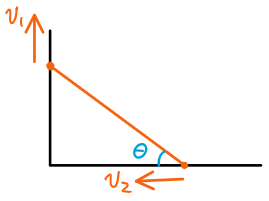
\includegraphics[width=5cm]{./figures/rod1.png}
\caption{杆的运动} \label{rod_fig1}
\end{figure}
如\autoref{rod_fig2}, 杆的两端被固定在两个垂直的轨道上运动, 两端的运动速度分别为 $v_1, v_2$, 已知杆与水平轨道的夹角为 $\theta$, 求 $v_1$ 和 $v_2$ 的关系.

解: 由\autoref{rod_eq3}, 两速度在杆方向的分量应该相等, 即
\begin{equation}
v_2 \cos\theta = v_1 \sin\theta
\end{equation}
即
\begin{equation}
v_2 = v_1 \tan\theta
\end{equation}
\end{exam}

\begin{exam}{人拉船模型}
\begin{figure}[ht]
\centering
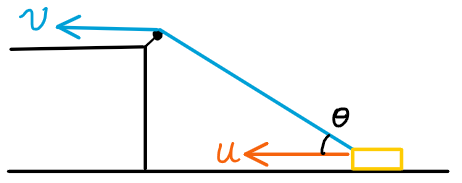
\includegraphics[width=5.3cm]{./figures/rod3.png}
\caption{人拉船模型} \label{rod_fig3}
\end{figure}
如\autoref{rod_fig3}, 人在岸上通过一小滑轮用绳子以速度 $v$ 拉船, 绳子与水平面的夹角为 $\theta$, 求船的速度 $u$.

解: 我们可以把从滑轮到船的这段绳子的长度缩短的速度用\autoref{rod_eq6} 来计算, 这个速度也就是人的速度
\begin{equation}
v = -\dv{L}{t} = u \cos\theta
\end{equation}
所以
\begin{equation}
u = \frac{v}{\cos\theta}
\end{equation}
\end{exam}

\subsubsection{角速度}
若已知两端点的速度, 如何求出角速度呢?

结论(过程未完成):
\begin{equation}\label{rod_eq4}
\bvec \omega = \frac{\uvec r}{r} \cross (\bvec v_2 - \bvec v_1)
\end{equation}

\subsubsection{加速度约束}
若我们想知道对加速度的约束, 只需对\autoref{rod_eq1} 两边再求一次时间导数, 即\autoref{rod_eq2} 的二阶时间导数.
\begin{equation}
\dv[2]{t} (\bvec r_2 - \bvec r_1)^2 = (\bvec v_2 - \bvec v_1)^2 + (\bvec r_2 - \bvec r_1) \vdot (\bvec a_2 - \bvec a_1) = 0
\end{equation}

结论(过程未完成):
\begin{equation}\label{rod_eq5}
\bvec a_1 \vdot \uvec r - \bvec a_2 \vdot \uvec r  = \omega^2 r
\end{equation}
$\omega$ 是杆的瞬时角速度的大小.

\begin{exam}{}
\begin{figure}[ht]
\centering
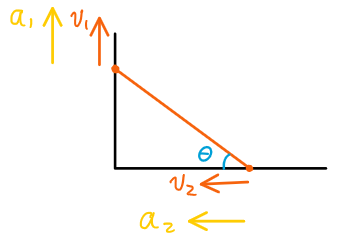
\includegraphics[width=5cm]{./figures/rod2.png}
\caption{杆的运动} \label{rod_fig2}
\end{figure}
在\autoref{rod_ex1} 的模型中, 若已知端点的速度 $v_1, v_2$ 和 $\theta$, 求两点加速度 $a_1, a_2$ 的关系.

解: 由\autoref{rod_eq4} 和\autoref{rod_eq5} 得,
\begin{equation}
\omega = (v_2 \cos\theta + v_1 \sin\theta)/r
\end{equation}
\begin{equation}
a_2 \cos\theta - a_1 \sin\theta = \omega^2 r = (v_2 \cos\theta + v_1 \sin\theta)^2/r
\end{equation}
\end{exam}

\subsection{动力学}
\pentry{转动惯量\upref{RigRot}}
轻杆没有质量, 也没有转动惯量. 假设我们只能在轻杆的两端对其施加两个力 $\bvec F_1, \bvec F_2$, 这两个力会满足什么条件呢? 首先, 轻杆受到的合力必须为 $\bvec 0$, 否则他就会马上被加速到无限快. 这意味着这两个力大小相等, 方向相反($\bvec F_1 + \bvec F_2 = \bvec 0$). 其次, 它受到的和力矩必须也为 $\bvec 0$, 否则就会瞬间拥有无限大的角速度. 这意味着两个力必须共线, 即都延杆的方向. 于是我们可以令 $\bvec F_1 = F \uvec r$, $\bvec F_2 = -F \uvec r$.

现在, 无论轻杆如何运动, 这两个力对轻杆做功的功率为
\begin{equation}
P = \bvec F_1 \vdot \bvec v_1 + \bvec F_2 \vdot \bvec v_2 = F (\uvec r \vdot \bvec v_1 - \uvec r \vdot \bvec v_2)
\end{equation}
由\autoref{rod_eq3} 可知功率恒为 0.
